\documentclass[9pt,twocolumn,twoside]{../../styles/osajnl}
\journal{i524} 

\title{Apache Tez- Application Data processing Framework}

\author[1]{Abhijt Thakre}

\affil[1]{School of Informatics and Computing, Bloomington, IN 47408, U.S.A.}
\affil[2]{Mechanical Engineer,Nagpur University, 2003}

\affil[*]{Corresponding authors: abhijit.thakre@gmail.com}

\dates{project-000, \today}

\ociscodes{Cloud, I524}

% replace this with your url in github/gitlab
\doi{\url{https://github.com/cloudmesh/classes/blob/master/docs/source/format/report/report.pdf}}

\begin{abstract}
There are lot of advancement in Hadoop framework from Hadoop1.0 to Hadoop 2.0. 
Hadoop 2.0 is layered architecture provides the YARN layer responsible for the resource management opens up the gate for developing different application engines on top of it. 
Apache Tez is one of such open source framework build on the top of YARN designed to build data-flow driven runtimes. 
This paper focusses mostly on introduction to Apache Tez framework. It provides the insight of the architecture used in building Tez. It also tried to cover the technologies using apache Tez as unifying framework and performance improvement achieved due to that.
\end{abstract}

\begin{document}

\maketitle

\section{Introduction}
 
In order to understand Tez as an framework we need to first dig into the history of Hadoop. Hadoop 1.0 have MapReduce as the central execution engine of its application. Any type of problem statement for analysis needs to be restructured to fit it to the map-reduce paradigm. 
It was also responsible for resource management and resource allocation. With Hadoop 2.0  these responsibilities got divided separately where YARN got the responsibility of general purpose resource management.

\begin{figure}[htbp]
\centering
\fbox{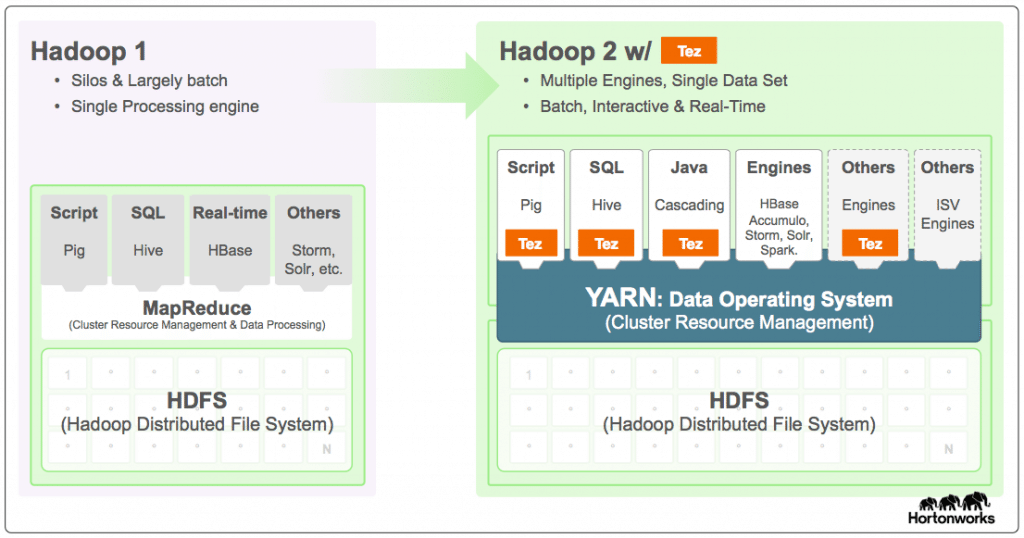
\includegraphics[width=\linewidth]{images/tez_architecture}}
\caption{\cite{www-tez.org}}
\label{Reference:false-color}
\end{figure}

Apache Hive, Apache PIG , CASCADING which was initially using Hadoop1 now run on Hadoop2 on YarN. These listed data processing application including map reduce have certain set of requirement from the  hadoop cluster in order to run efficiently. This is where Tez came in picture. Tez takes care of running the data processing application's efficiency and performance leaving the end user to only concentrate on the business logic.

\section{Tez Terminology}

 DAG -- Direct Acyclic Graphs, it represent overall job.  
 Vertex -- Logical step in processing. It contains the details of user logic and dependent environment.
 Task --   There can be multiple task in unit of work that vertex perform. 
 Edge --  This represents connection between producer and consumer vertices.


\section{Architecture and Implementation}

Tez was designed keeping in mind to address the problems which were not resolved by Hadoop. 
It was not build from the scratch but on the top of YARN layer to leavarage the 
advantages and work that were done for years on Hadoop. So Tez leavarage the discrete task based compute model,concept of data shuffling in map reduce,resource tentancy and
multi-tenancy model and build in security from Hadoop . 

Tez focuses mainly on below problem in addition.

\begin{itemize}
\item Without Tez, all the algorithm those needs to be executed on clusters needs to somehow translated to map-reduce api. This was impacting the efficiency and performance.However with Tez can naturally map the algorithm to execution engine in cluster.
        
\item Tez provide additionally interface for various application and technology for data source and syncing.

\item Performance.
\end{itemize}	


\section{TEZ-API}

Tez provides below two API for defining the data processing. 

\subsection{ DAG API}
	This API lets user define the structure for the computation.
	It lets user define the producer and consumers and how they talk to each other.
	This class of data processing application is represented as direct acyclic graphs 	

\subsection{RUNTIME API}
 	
	Using this API Layer Tez invokes the user code. This is where the actual code in the task  
to be executed is defined.


\section{Application Using Tez}

     Below are the product those are updated to be used on TEZ framework to run on YARN.
 
               
\subsection{Apache MapReduce}
      
    MapReduce is simple but powerful way of data processing. Tez product comes with
    build in map-reduce support.The configuration needs to be updated on YARN cluster
    for map reduce. Tez has inbuild map processor and reduce processor which provides the
    respective map reduce functionality.
               
 \subsection{Apache PIG}              
              
   PigLatin is the scripting language provided by Apache PIG used to write complex ETL.
   Tez API can handle the multiple output which is usually the case for the procedural language like PIGlatin, helps in keeping the code clean and maintainable.
 
  \subsection{Apache Hive}
              
   Apache Hive is used to convert the query written in HiveQL to map reduce and execute on hadooop cluster.The HiveQL is translation into map reduce format is often inefficient. Hive 0.13 was developed using Tez integration \cite{www-hive1} and the trees translate directly into DAGS.Hive0.14 have additional improvements like dynamic partition prunning. 
               
 \subsection{Apache Spark}
         
  Aparche spark provides scaLA API for distributed data processing. The output of the spark is DAG of tasks that performance distributed computation. The end output of Apache spark i.e Spark DAG is successfully converted and executed using Tez API.


 \section{Complex HIVE/PIG job running on MR vs TEZ}


 API library, YARN application master and runtime library are three major pillar used 
 by apache Tez project.Tez application DAG represents the flow of the application with input and 
 output as key-value pair for ease of use.


 Tez leavarage all the best ways used in distributed data processing 
 application for improving the efficient and performance. To quote few mechanism Tez uses
 like running the task close to its data,monitoring of slaggered task and running them in parallel
 to take them to finish, reusing the contain and sessions. 

 The following figure depicts, earlier running complex script and queries on Map Reduce use to take multiple jobs. 
 Running those job on Tez have reduced the number of steps. 
    

 \begin{figure}[htbp]
 \centering
 \fbox{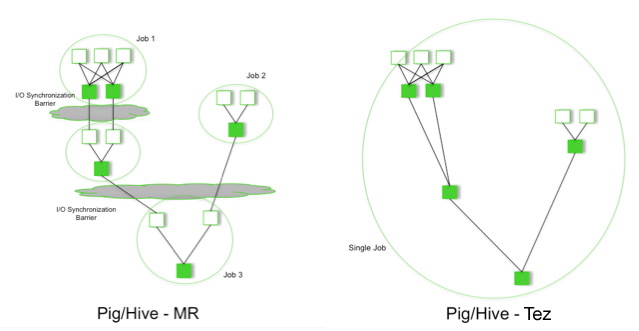
\includegraphics[width=\linewidth]{images/tez_perf}}
 \caption{\cite{www-tez.org}}
 \label{Reference:false-color}
 \end{figure}

 
 \section{Performance Results}

 Various test have been conducted to measure the performance of Hive and Pig implemented on the top of Tez vs its original    implementation on the Yarn. The below section details the configuration and test results for both of them.
 
 \subsection{HIVE}
 
 TEZ provides features like broadcast edges, runtime re-configuration and custom vertex manager which improves the overall 
 performance  of the Hive. The figure below depicts the comparison for Hive running on TEZ vs old map reduce implementation
 for the work load of 30 tb scale on 20 nodes clusters on 16 cores. Each node was assigned 256 Gb RAM and 6* 4 TB drives.

 \begin{figure}[htbp]
 \centering
 \fbox{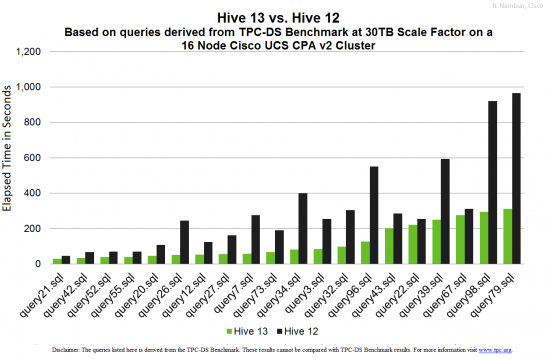
\includegraphics[width=\linewidth]{images/tez_perf1}}
 \caption{\cite{www-tez.org}}
 \label{Reference:false-color}
 \end{figure}
 
 One of the test results published in San Jose Hadoop Summit shows that Hive with Tez outperforms for TPC-H workload as compared
 to Hive with Map Reduce \cite{www-hivetest1}.
 
 \subsection{PIG}
 
 Yahoo have conducted production for complex ETL job.   The load used for testing encompass
 1.100K Task
 2.Input in TBs
 3.Complex DAGs.
 4.Combination of complex queries.

 The configuration of  environment/clusters used for the test
 1.Cluster has 4200 server 
 2.46PB hdfs storage
 3.90TB aggregate memory
 4.24GB RAM
 5.2x Xeon 2.40GHz , 6*2TB SATA on Hadoop 2.5, RHEL 6.5

 \begin{figure}[htbp]
 \centering
 \fbox{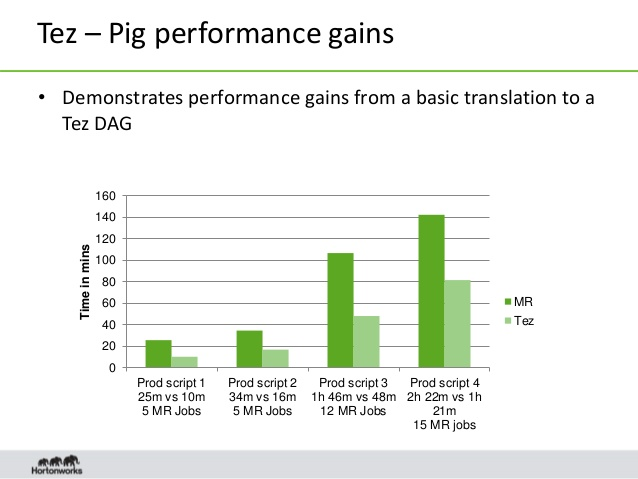
\includegraphics[width=\linewidth]{images/pig_perf}}
 \caption{\cite{www-tez.org}}
 \label{Reference:false-color}
 \end{figure}

 
 The performance improvement   150 to 200\% is observed with TEZ.
 
 
  \subsection{Spark Multi-Tenancy Test}
 
   Tez allocates the resources based on task as compared to YARN which allocated based on the job life cycle. 
   Spark on TEZ implementation have shown considerable speed up as the idle resource in TEZ based implementation get allocated 
   to next job as compared to the service based where the resource wait till the life cycle end . This has been proved based 
   on the 4- user concurrency test of partitioning a TPC-H lineitem data set. The allocation graph is shown in figure 5 and 6.
   

  \begin{figure}[htbp]
  \centering
  \fbox{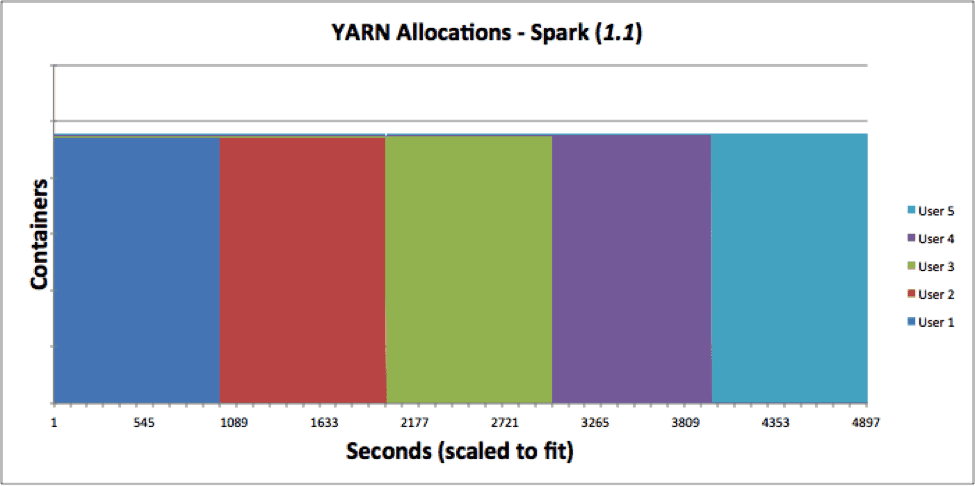
\includegraphics[width=\linewidth]{images/spark1.png}}
  \fbox{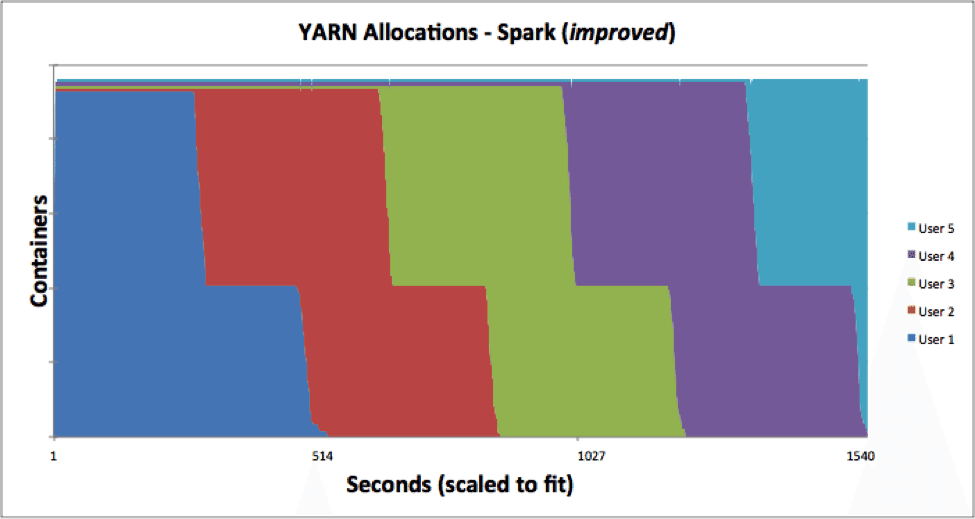
\includegraphics[width=\linewidth]{images/spark2.png}}
  \caption{\cite{www-spark1}}
  \centering
  \end{figure}
 
 
  \section{Conclusion} 

  With growing trend of big data and its processing, Hadoop has been in demand. Tez is open source architecture build
  modeling the data processing as direct acyclic graphs. 

  It has leverages all the strong points from Hadoop and addressed the issues which were concerning to the performance.

  Various examples discussed in paper shows how the implementation of various systems like HIVE,PIG, SPARK on TEZ have 
  shown substantial performance improvement as compared to the traditional MR api.
  Tez is open source and high customizable framework. It allows researchers and open source developer to integrate test their code. 
  


 \newpage

% Bibliography

\bibliography{references}
 
\section*{Author Biographies}
\begingroup
\setlength\intextsep{0pt}
\begin{minipage}[t][3.2cm][t]{1.0\columnwidth} % Adjust height [3.2cm] as required for separation of bio photos.
  \begin{wrapfigure}{L}{0.25\columnwidth}
    
\includegraphics[width=0.25\columnwidth]{images/john_smith.eps}
  \end{wrapfigure}
  \noindent
  {\bfseries Abhijit Thakre} received his BE (Mechanical) in 2003 from
  The University of Nagpur.
\end{minipage}
\endgroup


\appendix

\end{document}


\end{document}
